\subsubsection{Analisi al variare di N}
L'analisi delle prestazioni al variare del parametro N sono state svolte in 
condizioni di vario tipo, ma in ogni caso si osserva chiaramente che il tempo
impiegato decresce esponenzialmente all'aumentare dell'ampiezza della finestra
N.\\
Confrontando i due tipo di algoritmi, con timeout addatativo e non, si osserva
che per un timeout iniziale di 500 millisecondi, quello di tipo adattativo 
ottiene performance migliori in ogni caso, mentre per un timeout iniziale di 
250 millisecondi, che è il valore di soglia minimo, l'adattativo converge 
alla versione con timeout fisso solo in condizioni di basse e medie probabilità di 
perdita. In condizioni di perdite frequenti (70\%) ottiene performance peggiori ed 
in alcuni casi il grafico è soggetto a picchi. La causa di questo comportamento 
potrebbe essere legata al fatto che, in casi di perdite frequenti, si verificano
altrettanto frequentemente invii e e ritrasmissioni di un gran numero di pacchetti.
Questi eventi trattengono il servizio di invio impegnato abbastanza a lungo,
essendo inoltre operazioni di scrittura su file (socket), da
ritardare il timestamp relativo all'arrivo di eventuali ack, con conseguente 
errore sul calcolo dell'RTT e quindi aumento del timeout.
\begin{figure}[!hp]
	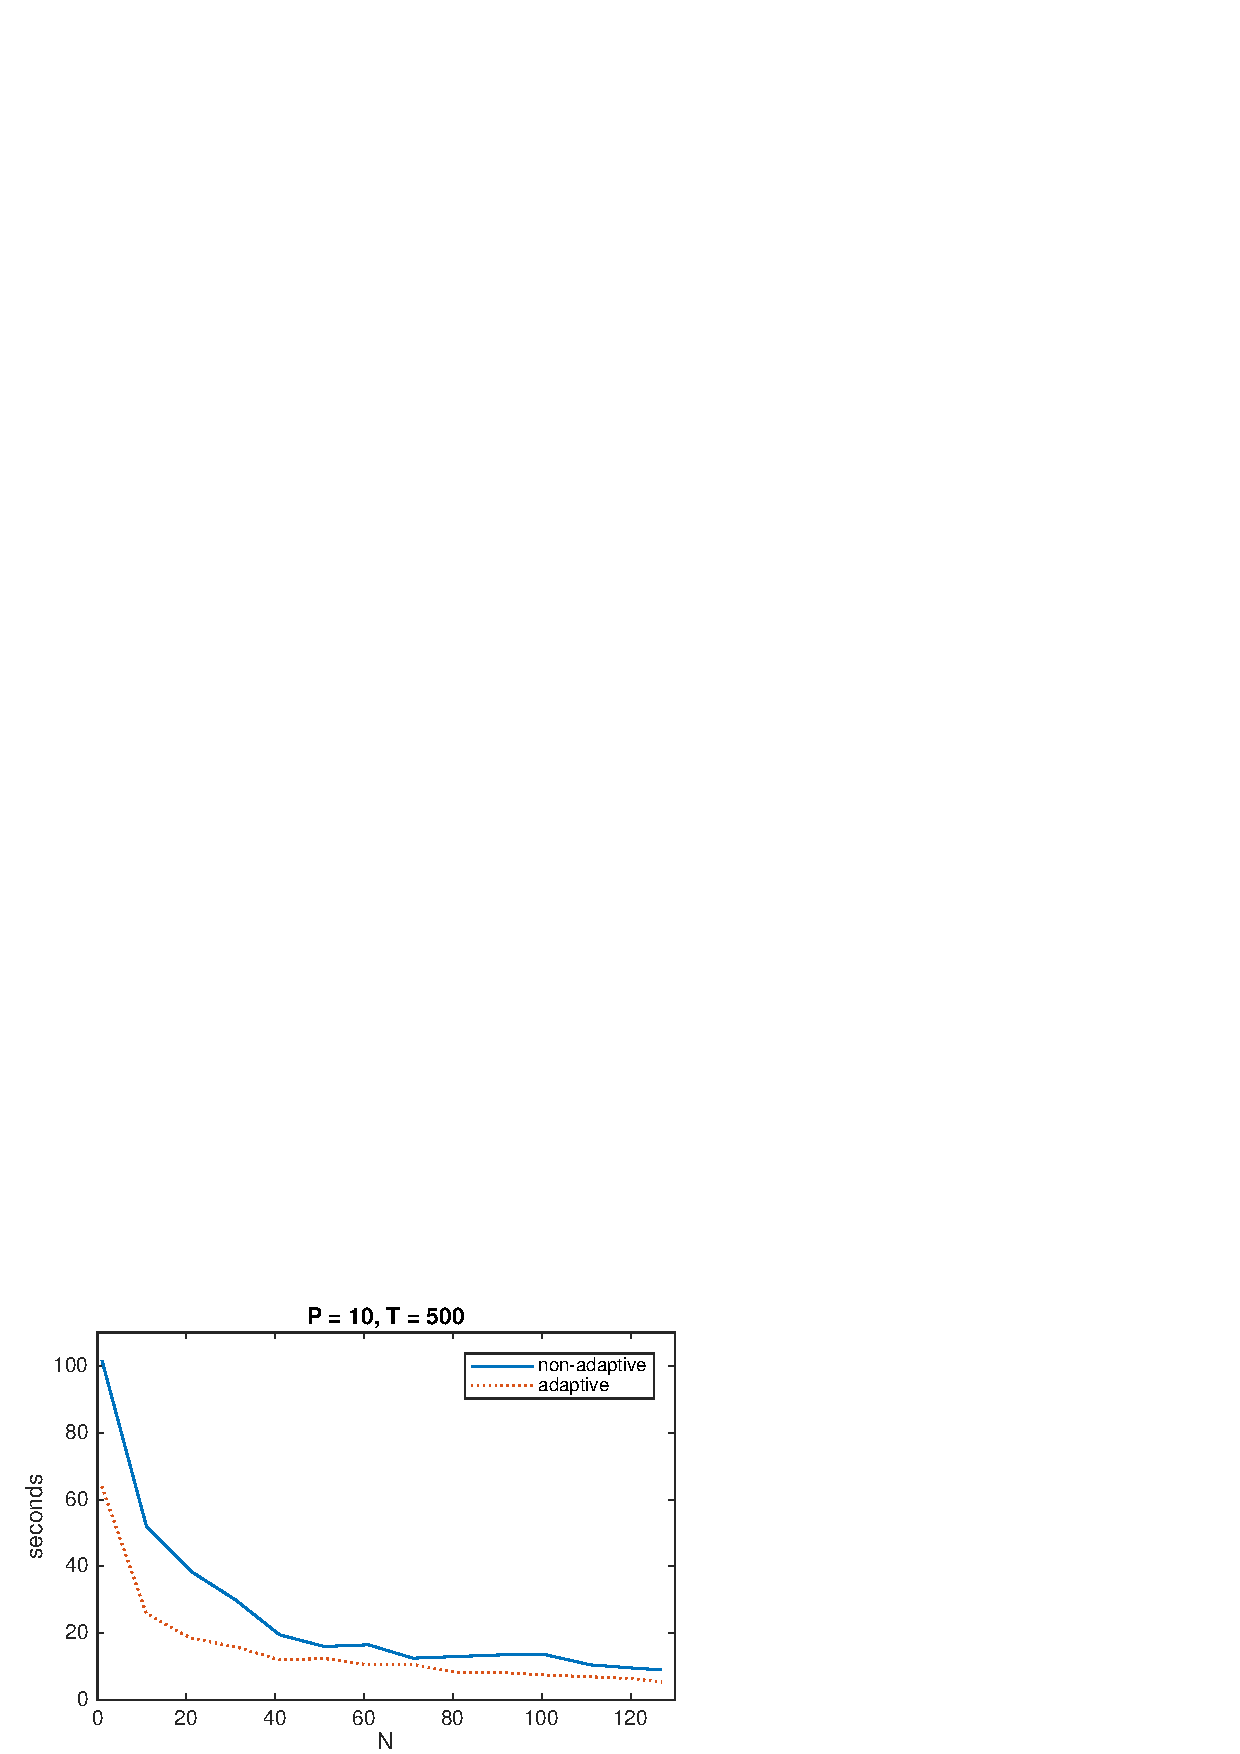
\includegraphics[scale=0.5]{images/N_T500_P10}
	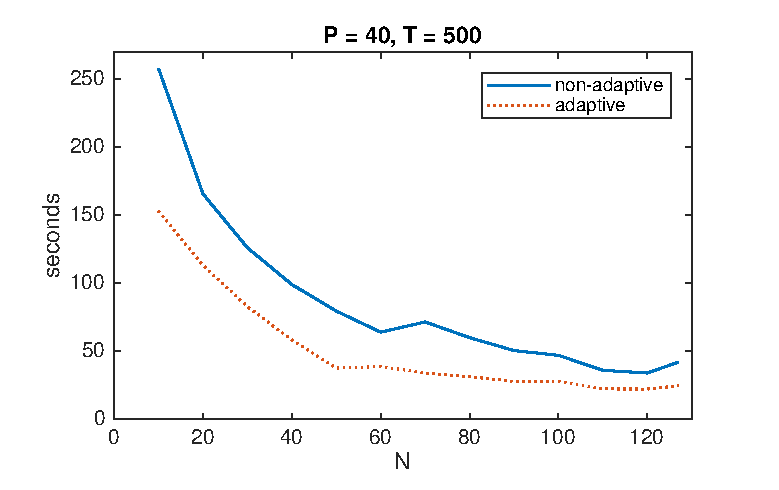
\includegraphics[scale=0.5]{images/N_T500_P40}
	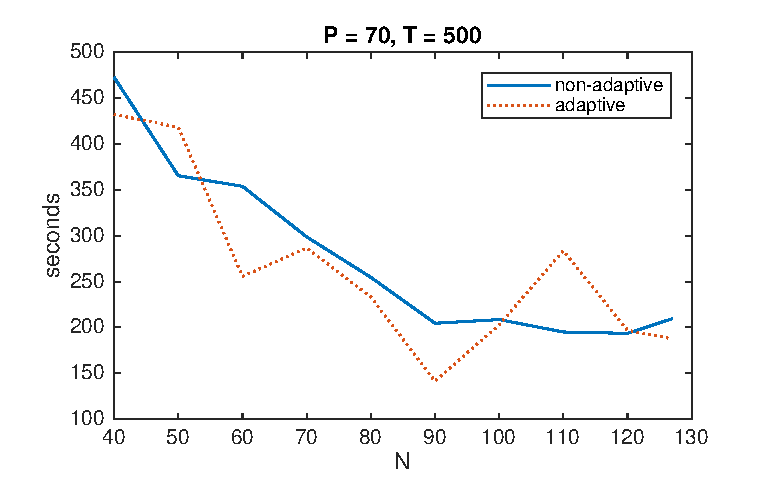
\includegraphics[scale=0.5]{images/N_T500_P70}
	\caption{prestazioni al variare dell'ampiezza della finestra N,
			 timeout T = 500 ms, probabilità di perdita bassa (P = 10\%),
			 media (P = 40\%) e alta (P = 70\%)}
\end{figure}
\begin{figure}[!hp]
	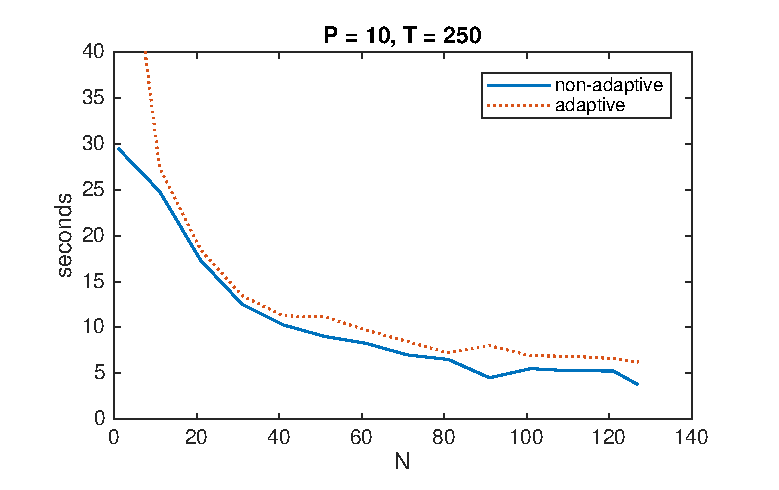
\includegraphics[scale=0.5]{images/N_T250_P10}
	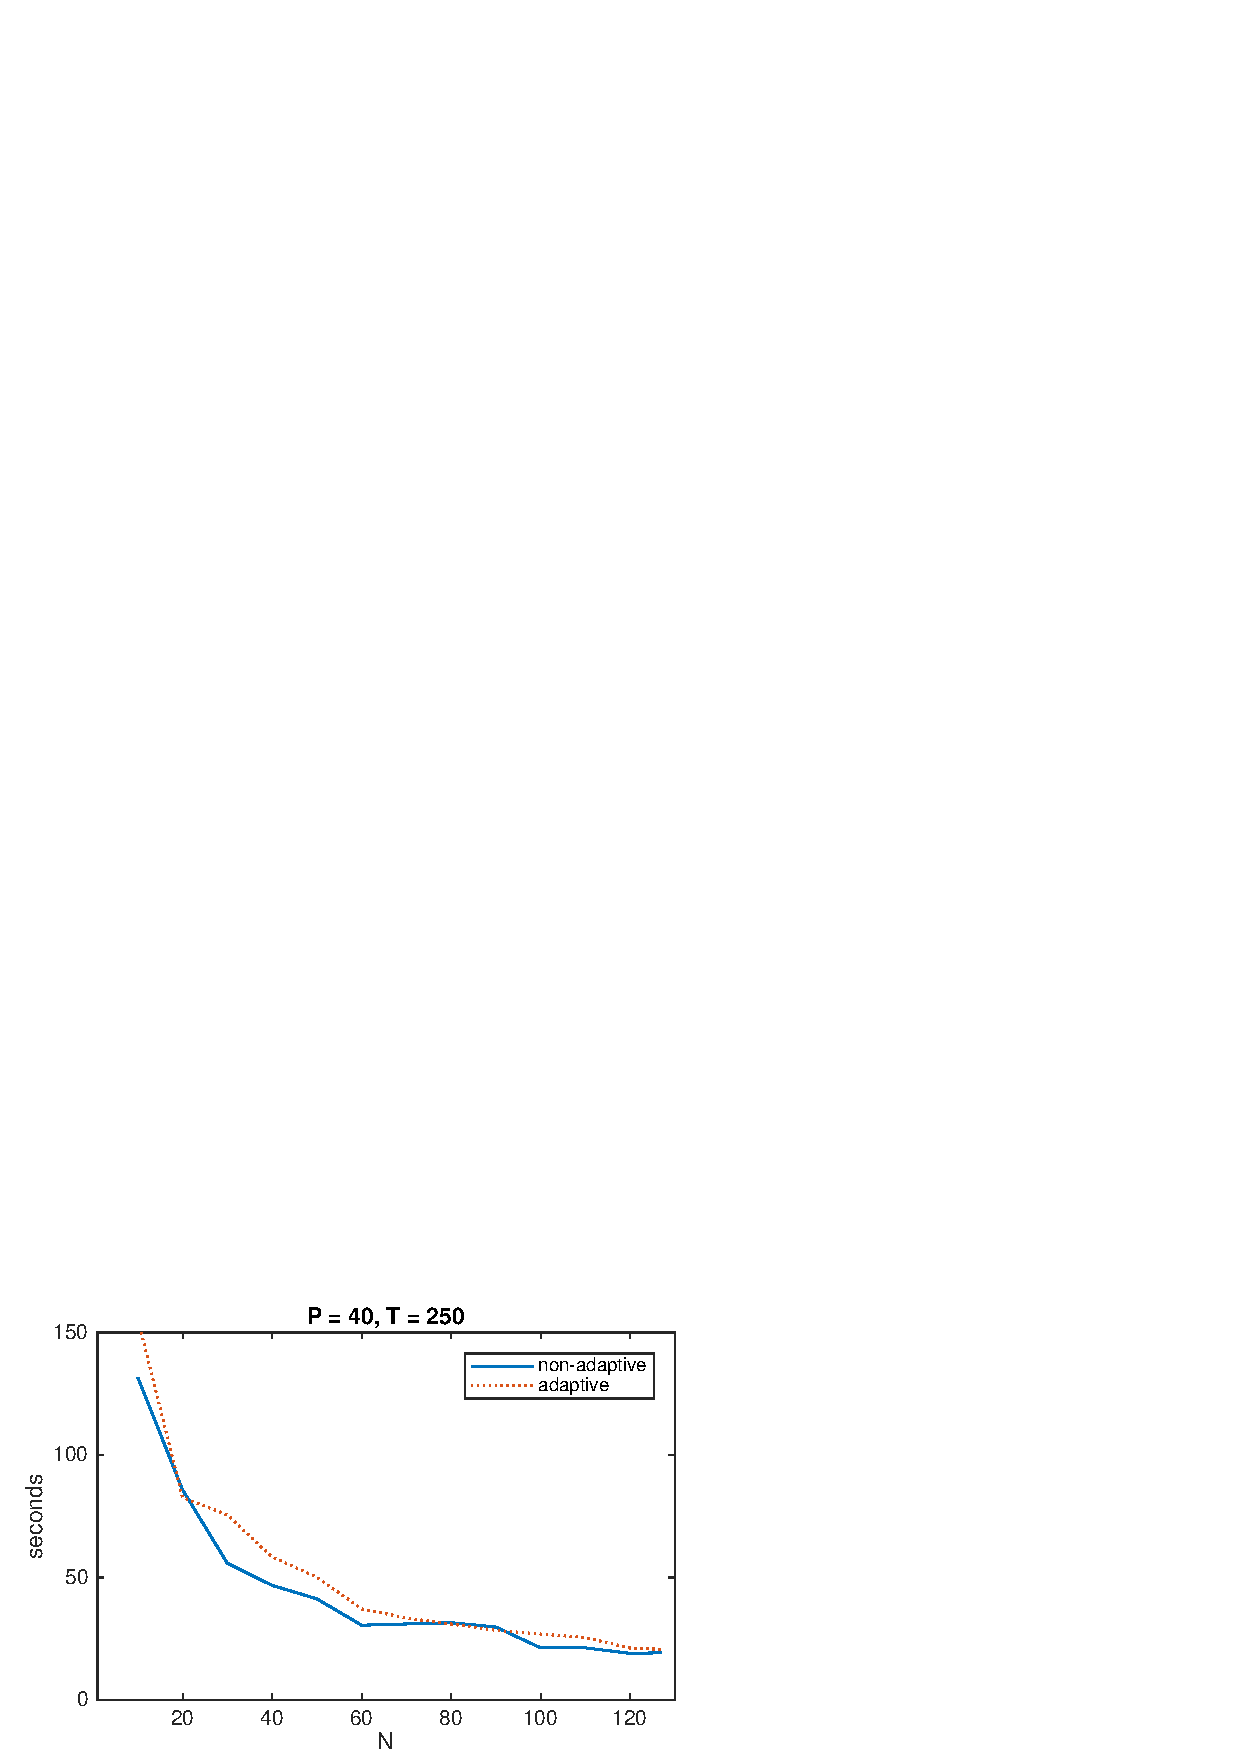
\includegraphics[scale=0.5]{images/N_T250_P40}
	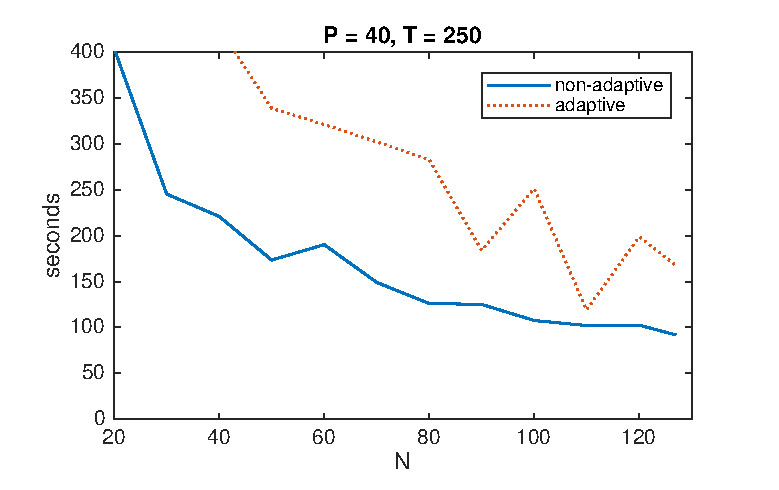
\includegraphics[scale=0.5]{images/N_T250_P70}
	\caption{prestazioni al variare dell'ampiezza della finestra N,
			 timeout T = 250 ms, probabilità di perdita bassa (P = 10\%),
			 media (P = 40\%) e alta (P = 70\%)}
\end{figure}
